\documentclass[border=10pt]{standalone}
\usepackage{tikz}
\usetikzlibrary{arrows.meta, decorations.markings, calc, positioning}

\tikzset{
  stitch node/.style={circle, draw, fill=white, inner sep=2pt,
                      minimum size=14pt, font=\footnotesize},
  knit node/.style={stitch node, fill=blue!10},
  purl node/.style={stitch node, fill=red!10},
  h edge/.style={thick, blue!60},
  v edge/.style={thick, red!60},
  yarn/.style={very thick, orange!80!black,
               decoration={markings,
                 mark=at position 0.55 with {\arrow{Stealth[length=4pt]}}},
               postaction={decorate}},
  yarn label/.style={font=\tiny, fill=white, inner sep=1pt, opacity=0.9,
                     text opacity=1},
  crossing over/.style={line width=3pt, white, line cap=round},
  crossing strand/.style={very thick, purple!70!black},
  over marker/.style={circle, fill=green!20, draw=green!60!black,
                      minimum size=8pt, inner sep=0pt, font=\tiny},
  under marker/.style={circle, fill=yellow!20, draw=yellow!60!black,
                       minimum size=8pt, inner sep=0pt, font=\tiny},
}

\begin{document}

% ============================================================
% Knitting Visualization: Three Graph Layers
% Pattern: 16 stitches, 4 rows, topology: flat
% ============================================================
%
% 1. STITCH GRAPH: one vertex per stitch, undirected edges
%    - Blue (h) edges: horizontal (within-row adjacency)
%    - Red (v) edges: vertical (row-to-row, through old loop)
%
% 2. YARN GRAPH: directed multigraph following the continuous yarn
%    - Orange arrows: yarn path in sequential creation order
%    - Curved edges: yarn wrapping around fabric selvage between rows
%    - Edge labels: position along the yarn
%
% 3. CROSSING DIAGRAM: yarn crossing presentation
%    - Orange: working yarn path
%    - Purple: old-loop strands (vertical connections)
%    - Green (+): knit crossing (working yarn under old loop)
%    - Yellow (-): purl crossing (working yarn over old loop)

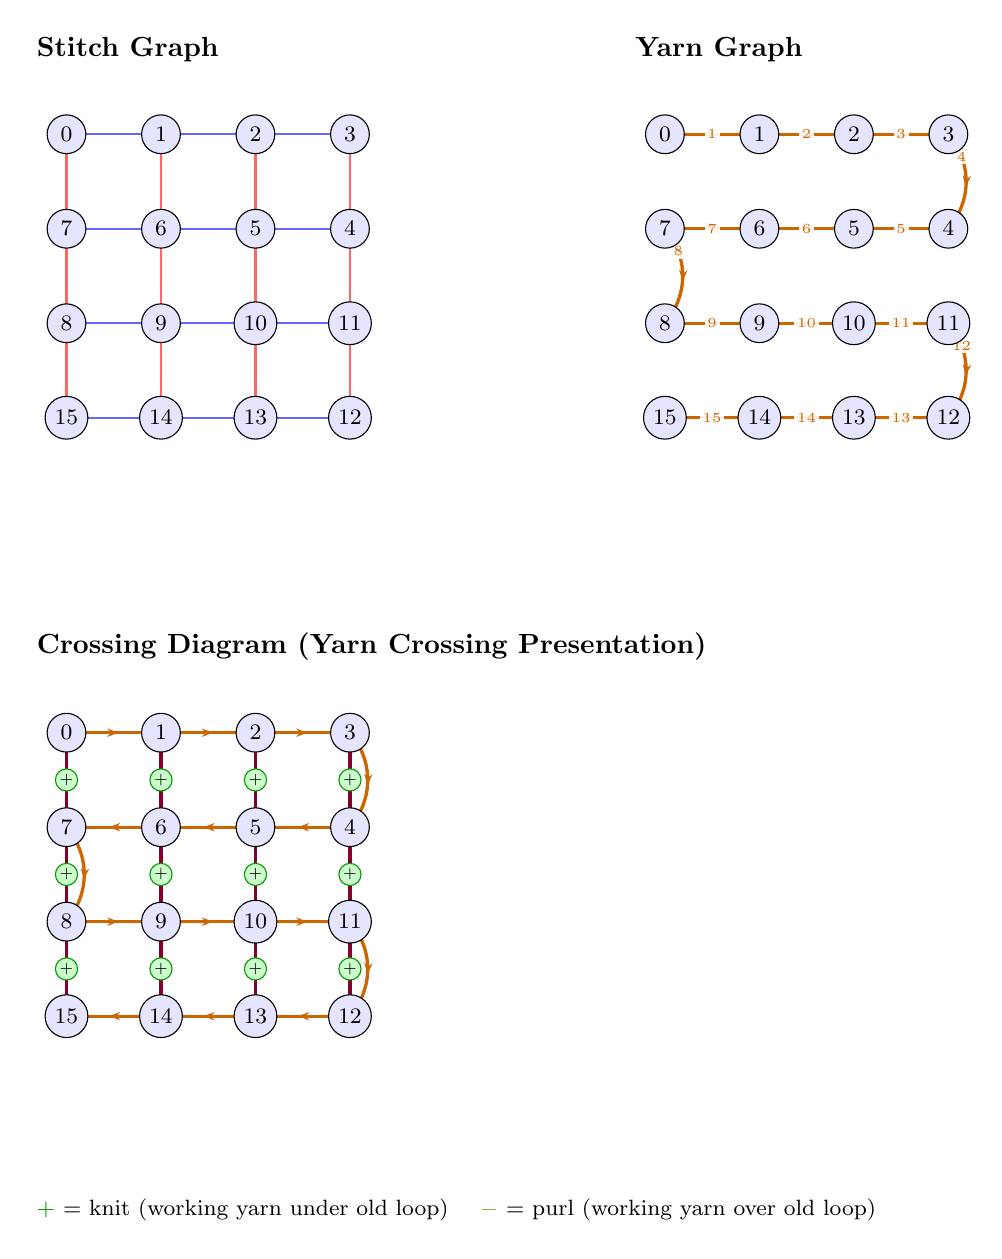
\begin{tikzpicture}[scale=1]
  % --- Stitch Graph ---
  \node[anchor=south west, font=\bfseries] at (-0.50,0.80) {Stitch Graph};
  \draw[h edge] (1.20,0.00) -- (0.00,0.00);
  \draw[h edge] (2.40,0.00) -- (1.20,0.00);
  \draw[h edge] (3.60,0.00) -- (2.40,0.00);
  \draw[v edge] (3.60,0.00) -- (3.60,-1.20);
  \draw[h edge] (2.40,-1.20) -- (3.60,-1.20);
  \draw[v edge] (2.40,0.00) -- (2.40,-1.20);
  \draw[h edge] (1.20,-1.20) -- (2.40,-1.20);
  \draw[v edge] (1.20,0.00) -- (1.20,-1.20);
  \draw[h edge] (0.00,-1.20) -- (1.20,-1.20);
  \draw[v edge] (0.00,0.00) -- (0.00,-1.20);
  \draw[v edge] (0.00,-1.20) -- (0.00,-2.40);
  \draw[h edge] (1.20,-2.40) -- (0.00,-2.40);
  \draw[v edge] (1.20,-1.20) -- (1.20,-2.40);
  \draw[h edge] (2.40,-2.40) -- (1.20,-2.40);
  \draw[v edge] (2.40,-1.20) -- (2.40,-2.40);
  \draw[h edge] (3.60,-2.40) -- (2.40,-2.40);
  \draw[v edge] (3.60,-1.20) -- (3.60,-2.40);
  \draw[v edge] (3.60,-2.40) -- (3.60,-3.60);
  \draw[h edge] (2.40,-3.60) -- (3.60,-3.60);
  \draw[v edge] (2.40,-2.40) -- (2.40,-3.60);
  \draw[h edge] (1.20,-3.60) -- (2.40,-3.60);
  \draw[v edge] (1.20,-2.40) -- (1.20,-3.60);
  \draw[h edge] (0.00,-3.60) -- (1.20,-3.60);
  \draw[v edge] (0.00,-2.40) -- (0.00,-3.60);
  \node[knit node] (s0) at (0.00,0.00) {0};
  \node[knit node] (s1) at (1.20,0.00) {1};
  \node[knit node] (s2) at (2.40,0.00) {2};
  \node[knit node] (s3) at (3.60,0.00) {3};
  \node[knit node] (s4) at (3.60,-1.20) {4};
  \node[knit node] (s5) at (2.40,-1.20) {5};
  \node[knit node] (s6) at (1.20,-1.20) {6};
  \node[knit node] (s7) at (0.00,-1.20) {7};
  \node[knit node] (s8) at (0.00,-2.40) {8};
  \node[knit node] (s9) at (1.20,-2.40) {9};
  \node[knit node] (s10) at (2.40,-2.40) {10};
  \node[knit node] (s11) at (3.60,-2.40) {11};
  \node[knit node] (s12) at (3.60,-3.60) {12};
  \node[knit node] (s13) at (2.40,-3.60) {13};
  \node[knit node] (s14) at (1.20,-3.60) {14};
  \node[knit node] (s15) at (0.00,-3.60) {15};
  % --- Yarn Graph ---
  \node[anchor=south west, font=\bfseries] at (7.10,0.80) {Yarn Graph};
  \draw[yarn] (7.60,0.00) -- (8.80,0.00)    node[yarn label, midway] {1};
  \draw[yarn] (8.80,0.00) -- (10.00,0.00)    node[yarn label, midway] {2};
  \draw[yarn] (10.00,0.00) -- (11.20,0.00)    node[yarn label, midway] {3};
  \draw[yarn, bend left=40] (11.20,0.00) to node[yarn label, near start] {4} (11.20,-1.20);
  \draw[yarn] (11.20,-1.20) -- (10.00,-1.20)    node[yarn label, midway] {5};
  \draw[yarn] (10.00,-1.20) -- (8.80,-1.20)    node[yarn label, midway] {6};
  \draw[yarn] (8.80,-1.20) -- (7.60,-1.20)    node[yarn label, midway] {7};
  \draw[yarn, bend left=40] (7.60,-1.20) to node[yarn label, near start] {8} (7.60,-2.40);
  \draw[yarn] (7.60,-2.40) -- (8.80,-2.40)    node[yarn label, midway] {9};
  \draw[yarn] (8.80,-2.40) -- (10.00,-2.40)    node[yarn label, midway] {10};
  \draw[yarn] (10.00,-2.40) -- (11.20,-2.40)    node[yarn label, midway] {11};
  \draw[yarn, bend left=40] (11.20,-2.40) to node[yarn label, near start] {12} (11.20,-3.60);
  \draw[yarn] (11.20,-3.60) -- (10.00,-3.60)    node[yarn label, midway] {13};
  \draw[yarn] (10.00,-3.60) -- (8.80,-3.60)    node[yarn label, midway] {14};
  \draw[yarn] (8.80,-3.60) -- (7.60,-3.60)    node[yarn label, midway] {15};
  \node[knit node] (y0) at (7.60,0.00) {0};
  \node[knit node] (y1) at (8.80,0.00) {1};
  \node[knit node] (y2) at (10.00,0.00) {2};
  \node[knit node] (y3) at (11.20,0.00) {3};
  \node[knit node] (y4) at (11.20,-1.20) {4};
  \node[knit node] (y5) at (10.00,-1.20) {5};
  \node[knit node] (y6) at (8.80,-1.20) {6};
  \node[knit node] (y7) at (7.60,-1.20) {7};
  \node[knit node] (y8) at (7.60,-2.40) {8};
  \node[knit node] (y9) at (8.80,-2.40) {9};
  \node[knit node] (y10) at (10.00,-2.40) {10};
  \node[knit node] (y11) at (11.20,-2.40) {11};
  \node[knit node] (y12) at (11.20,-3.60) {12};
  \node[knit node] (y13) at (10.00,-3.60) {13};
  \node[knit node] (y14) at (8.80,-3.60) {14};
  \node[knit node] (y15) at (7.60,-3.60) {15};
  % --- Crossing Diagram (Yarn Crossing Presentation) ---
  \node[anchor=south west, font=\bfseries] at (-0.50,-6.80) {Crossing Diagram (Yarn Crossing Presentation)};
  \draw[yarn] (0.00,-7.60) -- (1.20,-7.60);
  \draw[yarn] (1.20,-7.60) -- (2.40,-7.60);
  \draw[yarn] (2.40,-7.60) -- (3.60,-7.60);
  \draw[yarn, bend left=40] (3.60,-7.60) to (3.60,-8.80);
  \draw[yarn] (3.60,-8.80) -- (2.40,-8.80);
  \draw[yarn] (2.40,-8.80) -- (1.20,-8.80);
  \draw[yarn] (1.20,-8.80) -- (0.00,-8.80);
  \draw[yarn, bend left=40] (0.00,-8.80) to (0.00,-10.00);
  \draw[yarn] (0.00,-10.00) -- (1.20,-10.00);
  \draw[yarn] (1.20,-10.00) -- (2.40,-10.00);
  \draw[yarn] (2.40,-10.00) -- (3.60,-10.00);
  \draw[yarn, bend left=40] (3.60,-10.00) to (3.60,-11.20);
  \draw[yarn] (3.60,-11.20) -- (2.40,-11.20);
  \draw[yarn] (2.40,-11.20) -- (1.20,-11.20);
  \draw[yarn] (1.20,-11.20) -- (0.00,-11.20);
  \draw[crossing strand] (3.60,-7.60) -- (3.60,-8.80);
  \draw[crossing strand] (2.40,-7.60) -- (2.40,-8.80);
  \draw[crossing strand] (1.20,-7.60) -- (1.20,-8.80);
  \draw[crossing strand] (0.00,-7.60) -- (0.00,-8.80);
  \draw[crossing strand] (0.00,-8.80) -- (0.00,-10.00);
  \draw[crossing strand] (1.20,-8.80) -- (1.20,-10.00);
  \draw[crossing strand] (2.40,-8.80) -- (2.40,-10.00);
  \draw[crossing strand] (3.60,-8.80) -- (3.60,-10.00);
  \draw[crossing strand] (3.60,-10.00) -- (3.60,-11.20);
  \draw[crossing strand] (2.40,-10.00) -- (2.40,-11.20);
  \draw[crossing strand] (1.20,-10.00) -- (1.20,-11.20);
  \draw[crossing strand] (0.00,-10.00) -- (0.00,-11.20);
  \node[over marker] (cr0) at (3.60,-8.20) {+};
  \node[over marker] (cr1) at (2.40,-8.20) {+};
  \node[over marker] (cr2) at (1.20,-8.20) {+};
  \node[over marker] (cr3) at (0.00,-8.20) {+};
  \node[over marker] (cr4) at (0.00,-9.40) {+};
  \node[over marker] (cr5) at (1.20,-9.40) {+};
  \node[over marker] (cr6) at (2.40,-9.40) {+};
  \node[over marker] (cr7) at (3.60,-9.40) {+};
  \node[over marker] (cr8) at (3.60,-10.60) {+};
  \node[over marker] (cr9) at (2.40,-10.60) {+};
  \node[over marker] (cr10) at (1.20,-10.60) {+};
  \node[over marker] (cr11) at (0.00,-10.60) {+};
  \node[knit node] (c0) at (0.00,-7.60) {0};
  \node[knit node] (c1) at (1.20,-7.60) {1};
  \node[knit node] (c2) at (2.40,-7.60) {2};
  \node[knit node] (c3) at (3.60,-7.60) {3};
  \node[knit node] (c4) at (3.60,-8.80) {4};
  \node[knit node] (c5) at (2.40,-8.80) {5};
  \node[knit node] (c6) at (1.20,-8.80) {6};
  \node[knit node] (c7) at (0.00,-8.80) {7};
  \node[knit node] (c8) at (0.00,-10.00) {8};
  \node[knit node] (c9) at (1.20,-10.00) {9};
  \node[knit node] (c10) at (2.40,-10.00) {10};
  \node[knit node] (c11) at (3.60,-10.00) {11};
  \node[knit node] (c12) at (3.60,-11.20) {12};
  \node[knit node] (c13) at (2.40,-11.20) {13};
  \node[knit node] (c14) at (1.20,-11.20) {14};
  \node[knit node] (c15) at (0.00,-11.20) {15};
  \node[anchor=north west, font=\footnotesize] at (-0.5,-13.4) {
    \textcolor{green!60!black}{$+$} = knit (working yarn under old loop) \quad
    \textcolor{yellow!60!black}{$-$} = purl (working yarn over old loop)
  };
\end{tikzpicture}

\end{document}
